Una vez llegados a este punto, siempre es interesante comparar el resultado final con las aplicaciones que tomamos como referencia en un principio. Como ya se indicó en el capítulo dos, usamos como punto de partida tres aplicaciones que abarcan el campo del control remoto móvil.\\

\section{Funcionalidad}

Nuestro propósito inicial era mejorar ciertos aspectos de estas aplicaciones ya existentes, y en este apartado observamos resultados.

\subsection{Funcionalidades destacadas compartidas con VNC++}
\begin{itemize}
\item Hacer zoom.
\item Mostrar teclado.
\item Escribir.
\item Enviar secuencia de teclas.
\item Recuerda conexiones previas.
\end{itemize}
\subsection{Funcionalidades diferentes respecto VNC++}
\begin{itemize}
\item \textbf{RealVNC:} como ya se matizó, esta aplicación está basada en software privativo, por lo que no disponemos de mucha información relativa a la implementación interna de este proyecto. Pero algo que nos propusimos desde el principio era crear un software puramente libre ya que pensamos que es así como se llega a un producto final con más opciones de desarrollo y uso futuro.\\

Permite, a través de un menú de opciones, desactivar el modo de pantalla completa, así como opción de Copy\&paste. También es destacable la diferencia en el manejo, en VNC Viewer al mover el dedo por la pantalla lo que moveremos es el cursor y no la imagen como en nuestro caso.
\item \textbf{MultiVNC:} libre y de código abierto, usa aceleración hardware OpenGL para el dibujado y el zoom, mientras que en nuestro caso se ha optado por el uso de Canvas. El manejo en la pantalla de MultiVNC es igual que el de RealVNC.
\item \textbf{AndroidVNC} también es libre y de código abierto, pero como contrapartida tiene una interfaz pobre y además el usuario se ve obligado a tener la pantalla en posición horizontal. En dispositivos con pantallas de reducido tamaño, la información es difícil de acceder, haciéndose el manejo bastante incómodo. En contrapartida ofrece muchos métodos de control, así como, la posibilidad de enviar texto desde un campo de texto.
\end{itemize}
\subsection{Mejoras consideradas}

Nuestra principal meta, como se indica en la sección de objetivos(Sección 1.3), era lograr usar el potencial del NDK para el uso de VNC, que es la principal desventaja de todos los proyectos software libre estudiados.\\

Partiendo de esta diferencia, el resto de matices los hemos querido mejorar también, viendo las deficiencias que pudieran tener el resto de aplicaciones, que echamos en falta como usuarios.\\

Como todas ellas usamos el protocolo RFB, con opciones de pantalla completa, mostrar teclado, etc, con lo que en estos aspectos no mejoramos ni empeoramos nada.\\

Pero como usuarios hemos intentado hacer un envío más intuitivo de teclas combinadas(tipo Alt-F4), así como diálogos informativos al usuario. Además se ha incorporado la opción de centrar la imagen, con el fin de recolocarse.\\

En cuanto a la codificación de la imagen, los otros dos proyectos software de referencia usan ZRLE, lo que implica no aplicar ningún tratamiento previo a la imagen con la consiguiente carga en la transmisión de datos. VNC++, sin embargo, usa codificación Tight, que aplica una compresión a la imagen para tener un rendimiento mayor.\\

Otro logro significativo es que nuestra aplicación soporta SSL(capa de conexión segura), que es un protocolo criptográfico que permite conexiones seguras, que es algo que como usuario siempre se demanda.\\

\section{Rendimiento}

Para analizar los resultados obtenidos, desde el punto de vista del rendimiento, se han querido analizar diferentes puntos: uso de CPU, tiempo de respuesta y uso de la red.

\subsection{Entorno de pruebas}

Para hacer la mediciones en un entorno adecuado, las pruebas han sido realizadas en el siguiente entorno:
\begin{itemize}
\item \textbf{Versión Android:} 4.2.2 Jelly Bean.
\item \textbf{Móvil:} Samsung Galaxy S3.
\item \textbf{Sistema Operativo en Servidor:} Linux Mint Debian Edition 64 Mate.
\item \textbf{Resolución del servidor:} 2704x1818.
\item \textbf{Servidor VNC:} X11vnc.
\item \textbf{Router:} Xavi 7968.
\end{itemize}
\newpage
Aplicaciones a comparar:
\begin{itemize}
\item VNC++.
\item RealVNC (VNC viewer).
\item AndroidVNC.
\item MultiVNC.
\end{itemize}

Para unas mediciones adecuadas, las pruebas se han realizado en una red local cerrada, en la cual, el servidor se encontraba conectado al switch mediante cable de ethernet y el móvil mediante wifi. También se han hecho las pruebas mediante el uso de 3G en móvil, en un entorno equivalente, con la excepción de que en este caso el Servidor se encontraba conectado a internet.

\subsection{Características de las pruebas}

En las pruebas se ha querido someter a las aplicaciones a una situación de estrés , para ello se ha llevado a cabo la reproducción de un vídeo en 1080p a pantalla completa durante aproximadamente 4 minutos (2 minutos en el caso del 3G). Las muestras tomadas a partir de las mismas son aproximadamente de los primeros 180 segundos (80 segundos con 3G) de la aplicación, partiendo desde el inicio total de la conexión. El vídeo se encontraba en reproducción desde el primer momento de la conexión.

\subsection{Resultados}

En el primer punto, uso de CPU, no se ha conseguido ninguna forma fiable de conseguir mediciones, y por otro lado, no todas las aplicaciones utilizan la misma tecnología, por ejemplo, MultiVNC utiliza GPU para la representación. Por ello se ha decidido desechar las pruebas relativas a este punto.\\

En segundo lugar, tiempo de respuesta, nos encontramos en un caso análogo al anterior, aunque en este caso si cabe destacar un matiz. En la carga inicial de la aplicación, al mostrar la primera imagen del servidor, en las pruebas con Wifi , RealVNC es sensiblemente más rápido que VNC++ y ambos son notablemente más rápidos que AndroidVNC, el cual a su vez, es sensiblemente más rápido que MultiVNC.\\

Cabe destacar que en el caso de conexión 3G las diferencias fueron muy significativas, mientras RealVNC y VNC++ mantuvieron tiempos parejos (como ya se ha descrito anteriormente), AndroidVNC y MultiVNC mostraron la primera imagen prácticamente al acabar la prueba.\\

En cuanto al tiempo de respuesta una vez hecha la carga, nos encontraríamos en rendimientos muy parejos entre todos, nada que destacar en este punto.\\

Por último nos encontramos en las pruebas de uso de red, en este punto si hemos podido obtener resultados fiables y concluyentes, por ello lo detallaremos de forma amplia en el siguiente punto.

\subsection{Uso de Red}

Para la realización de estas mediciones se ha utilizado el software Wireshark (Ver sección 1.1.10), mediante el cual se ha podido esnifar los paquetes, para posteriormente, recoger los resultados.\\

Antes de proceder con los resultados explicaremos los diferentes campos que componen los resultados:
\begin{itemize}
\item \textbf{Packets:} número de paquetes.
\item \textbf{Between first and last packet:} tiempo transcurrido desde el primer y último paquete.
\item \textbf{Avg. Packet/sec:} promedio de paquetes por segundo.
\item \textbf{Avg. Packet size:} promedio de tamaño del paquete.
\item \textbf{Bytes:} bytes totales de la conexión.
\item \textbf{Avg. bytes/sec:} promedio de bytes por segundo.
\item \textbf{Avg. Mbit/sec:} promedio de Megabits por segundo.
\end{itemize}

Dentro de las cuales encontraremos dos columnas:
\begin{itemize}
\item \textbf{Captured:} cálculos en función del total de paquetes capturados.
\item \textbf{Displayed:} cálculos en función de los paquetes que se muestran, esto es, con filtros aplicados.
\end{itemize}

Para el análisis nos fijaremos en la columna Displayed ya que ésta representa los cálculos con el filtro de 180 segundos aproximadamente, como se podrá observar. De entre los campos, los que tendrán más relevancia y peso para las pruebas son Avg bytes/sec y Avg. Mbit/sec, ya que el cálculo promedio muestra resultados de mayor relevancia.\\
\newpage
Como ya hemos nombrado anteriormente, las mediciones se han hecho en dos situaciones, Wifi y 3G, los resultados son:\\

\textbf{Wifi:}\\

VNC++:
\begin{figure}[h]
\begin{flushleft}
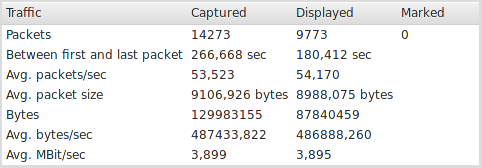
\includegraphics[scale=0.7]{vncppwifi.png}
\end{flushleft}
\caption{Rendimiento Wifi VNC++}
\end{figure}

RealVNC:
\begin{figure}[h]
\begin{flushleft}
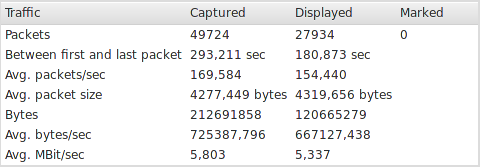
\includegraphics[scale=0.7]{realvncwifi.png}
\end{flushleft}
\caption{Rendimiento Wifi RealVNC}
\end{figure}

AndroidVNC:
\begin{figure}[h]
\begin{flushleft}
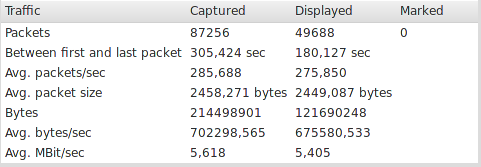
\includegraphics[scale=0.7]{androidvncwifi.png}
\end{flushleft}
\caption{Rendimiento Wifi AndroidVNC}
\end{figure}
\newpage
MultiVNC:
\begin{figure}[h]
\begin{flushleft}
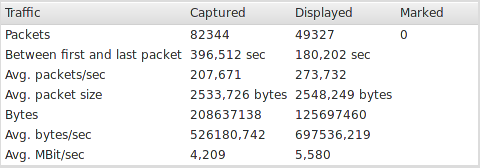
\includegraphics[scale=0.7]{multivncwifi.png}
\end{flushleft}
\caption{Rendimiento Wifi MultiVNC}
\end{figure}

Como se puede observar, los resultados de RealVNC, AndroidVNC y MultiVNC son muy parejos, esto es debido principalmente a que todos ellos utilizan la codificación para la imagen ZRLE. Sin embargo los resultados de VNC++ son muy distintos, debido a que usa Tight.\\

En primer lugar se puede observar que tanto AndroidVNC como MultiVNC tienen un tamaño medio de paquetes muy parecido, mientras que los de RealVNC son aproximadamente el doble, y a su vez, los de VNC++ el doble de este.\\

Por otro lado, encontramos que el promedio de Mbit/sec de RealVNC, AndroidVNC y MultiVNC es muy parecido pero el de VNC++ es significativamente inferior. Esto se debe a la codificación de la imagen, como ya dijimos anteriormente, la codificación usada por VNC++ es Tight. Esto provoca, al procesar previamente la imagen, que el uso de la red sea inferior.\\

De estos resultados se pueden concluir principalmente dos cosas:
\begin{itemize}
\item Por un lado, que debido a un uso inferior de la red, VNC++ funcionaría mejor en entornos de poca conexión.
\item Y por el otro, que debido a que los paquetes son más grandes, VNC++ respondería peor a la pérdida de paquetes, ya que si se pierde un paquete la información a reenviar es superior.
\end{itemize}
\newpage
\textbf{3G:}\\

VNC++:
\begin{figure}[h]
\begin{flushleft}
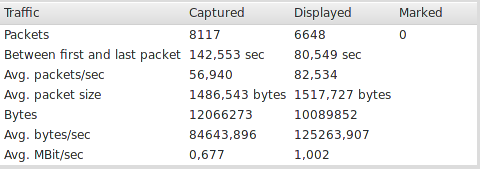
\includegraphics[scale=0.7]{vncpp3g.png}
\end{flushleft}
\caption{Rendimiento 3G VNC++}
\end{figure}

RealVNC:
\begin{figure}[h]
\begin{flushleft}
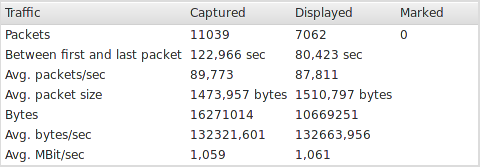
\includegraphics[scale=0.7]{realvnc3g.png}
\end{flushleft}
\caption{Rendimiento 3G RealVNC}
\end{figure}

AndroidVNC:
\begin{figure}[h]
\begin{flushleft}
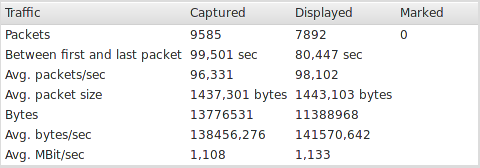
\includegraphics[scale=0.7]{androidvnc3g.png}
\end{flushleft}
\caption{Rendimiento 3G AndroidVNC}
\end{figure}
\newpage
MultiVNC:
\begin{figure}[h]
\begin{flushleft}
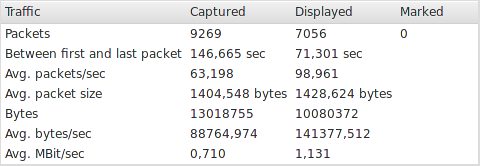
\includegraphics[scale=0.7]{multivnc3g.png}
\end{flushleft}
\caption{Rendimiento 3G MultiVNC}
\end{figure}

Como se puede observar los valores con una conexión 3G son muy parecidos, ello es debido a como funciona la propia conexión y sus limitaciones. Así pues se puede concluir que el rendimiento en entornos de 3G de las aplicaciones es equivalente. 
